\documentclass[a4paper,11pt,twoside]{scrartcl}
\usepackage[T1]{fontenc}
\usepackage{subcaption}
\usepackage[utf8]{inputenc}
\usepackage{ngerman, eucal, mathrsfs, amsfonts, bbm, amsmath, amssymb, stmaryrd,graphicx, array, geometry, color, wrapfig, float, hyperref, epstopdf,gensymb, subcaption, extarrows}
\geometry{left=25mm, right=15mm, bottom=25mm}
\setlength{\parindent}{0em} 
\setlength{\headheight}{0em} 
\title{Graphenalgorithmen\\ Blatt 8}
\author{Markus Vieth\and Christian Stricker}
\date{\today}
\input{../head/lstlisting.tex}
\usepackage{float}
\usepackage[section]{placeins}
\usepackage{epstopdf}
\usepackage{wrapfig}
\usepackage{caption}
\usepackage{subcaption}
\usepackage{graphicx}
\usepackage{pgfplots}
\usepackage[usenames,dvipsnames,svgnames,table]{xcolor}
\usetikzlibrary{plotmarks}
\usetikzlibrary{patterns}
\usetikzlibrary{decorations.pathmorphing}
\usetikzlibrary{calc}
\usetikzlibrary{shapes}
\newcommand{\coloredcircled}[3][black]{{\large \Large\color{#2}\textcircled {{\small\color{#1}#3}}}}% Circlecolor, Textcolor, text
\newcommand{\ddvec}[2]{\begin{pmatrix}#1\\#2\end{pmatrix}}
\newcommand{\dddvec}[3]{\begin{pmatrix}#1\\#2\\#3\end{pmatrix}}
\newcommand{\longvec}[1]{\overset{\longrightarrow}{#1}}
\newcommand{\eunorm}[1]{\left\lVert#1\right\rVert_2}
\newcommand{\scalar}[2]{\left<#1,#2\right>}\newcommand{\cor}[1]{\textcolor{red}{\textit{#1}}}
\newcommand{\qed}{%
	\begin{flushright}
		q.e.d.
	\end{flushright}%
	}
\begin{document}
\maketitle
\cleardoublepage
\pagestyle{myheadings}
\markboth{Markus Vieth, Christian Stricker}{Markus Vieth, Christian Stricker}

\newpage
\section{Aufgabe 1: Baumzerlegung (6 Punkte)}
\subsection{Graph a}
Ist keine Baumzerlegung, da 1 in keiner Tasche ist und somit die Node Coverage verletzt ist.
\subsection{Graph b}
Ist keine Baumzerlegung, da im Pfad $(123) -- (34) -- (46) -- (356)$ der Knoten $3$ zwar in der ersten und letzten Tasche aber nicht in $(46)$ ist und somit die Coherence verletzt ist.
\subsection{Graph c}
Kein Widerspruch gefunden $\Rightarrow$ valide Baumzerlegung
\subsection{Graph d}
Keine Baumzerlegung, da für die Kante $(4,8)$ keine Tasche existiert in der die Knoten $(4)$ und $(8)$ enthalten sind und somit die Edge Coverage verletzt ist.
\subsection{Graph e}
Kein Widerspruch gefunden $\Rightarrow$ valide Baumzerlegung
\section{Aufgabe 2: Max-Wheight-Independent-Set (MWIS) (10 Punkte)}
\begin{figure}[H]
	\centering
	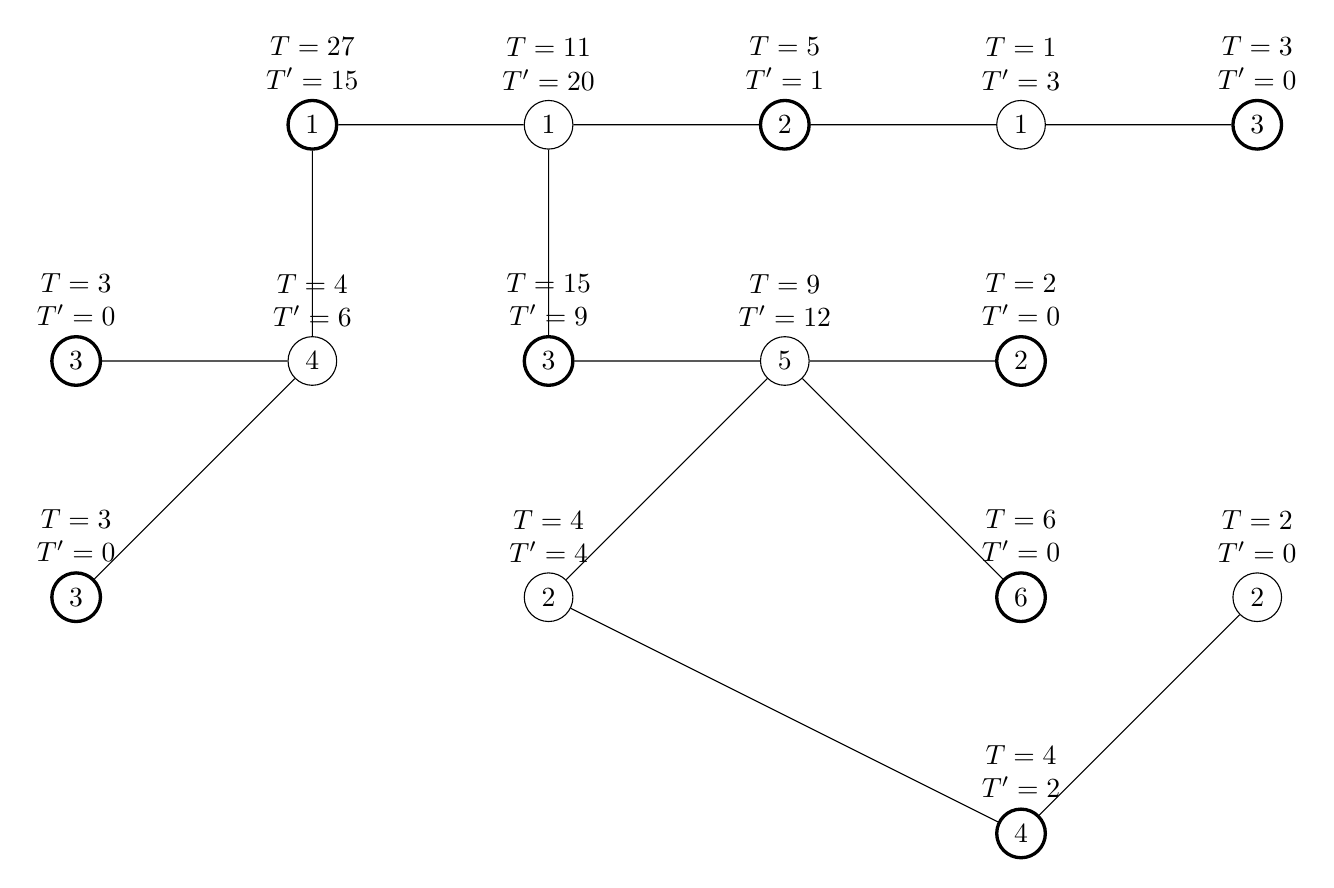
\begin{tikzpicture}[scale=3]
		\node[very thick, circle, draw, align=center, label={[align=center]90:{$T=27$\\$T'=15$}}] at ( 0, 0)  (1) {1};
		\node[circle, draw, align=center, label={[align=center]90:{$T=11$\\$T'=20$}}] at ( 1, 0)  (2) {1};
		\node[very thick, circle, draw, align=center, label={[align=center]90:{$T=5$\\$T'=1$}}] at ( 2, 0)  (3) {2};
		\node[circle, draw, align=center, label={[align=center]90:{$T=1$\\$T'=3$}}] at ( 3, 0)  (4) {1};
		\node[very thick, circle, draw, align=center, label={[align=center]90:{$T=3$\\$T'=0$}}] at ( 4, 0)  (5) {3};
		\node[circle, draw, align=center, label={[align=center]90:{$T=4$\\$T'=6$}}] at ( 0,-1)  (6) {4};
		\node[very thick, circle, draw, align=center, label={[align=center]90:{$T=3$\\$T'=0$}}] at (-1,-1)  (7) {3};
		\node[very thick, circle, draw, align=center, label={[align=center]90:{$T=3$\\$T'=0$}}] at (-1,-2)  (8) {3};
		\node[very thick, circle, draw, align=center, label={[align=center]90:{$T=15$\\$T'=9$}}] at ( 1,-1)  (9) {3};
		\node[circle, draw, align=center, label={[align=center]90:{$T=9$\\$T'=12$}}] at ( 2,-1) (10) {5};
		\node[very thick, circle, draw, align=center, label={[align=center]90:{$T=2$\\$T'=0$}}] at ( 3,-1) (11) {2};
		\node[circle, draw, align=center, label={[align=center]90:{$T=4$\\$T'=4$}}] at ( 1,-2) (12) {2};
		\node[very thick, circle, draw, align=center, label={[align=center]90:{$T=6$\\$T'=0$}}] at ( 3,-2) (13) {6};
		\node[circle, draw, align=center, label={[align=center]90:{$T=2$\\$T'=0$}}] at ( 4,-2) (14) {2};
		\node[very thick, circle, draw, align=center, label={[align=center]90:{$T=4$\\$T'=2$}}] at ( 3,-3) (15) {4};
		\draw (8)--(6)--(7) (6)--(1)--(2)--(3)--(4)--(5) (2)--(9) -- (10)--(11) (10)--(12)--(15)--(14) (10)--(13); 
	\end{tikzpicture}
\end{figure}
$\Rightarrow$ $MWIS=(27,\{\text{siehe markierte Knoten}\})$
\section{Aufgabe 3: MWIS (10 Punkt)}
\begin{figure}[H]
	\centering
	\begin{subfigure}{.3\textwidth}
		\centering
		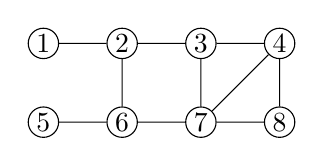
\begin{tikzpicture}
			\node[draw, circle, inner sep = 1] at (0,1) (1) {1};
			\node[draw, circle, inner sep = 1] at (1,1) (2) {2};
			\node[draw, circle, inner sep = 1] at (2,1) (3) {3};
			\node[draw, circle, inner sep = 1] at (3,1) (4) {4};
			\node[draw, circle, inner sep = 1] at (0,0) (5) {5};
			\node[draw, circle, inner sep = 1] at (1,0) (6) {6};
			\node[draw, circle, inner sep = 1] at (2,0) (7) {7};
			\node[draw, circle, inner sep = 1] at (3,0) (8) {8};
			\draw (1) -- (2) -- (3) -- (4) -- (8) --(7) --(6)--(5)
			(2) --(6) (3)--(7)--(4);
		\end{tikzpicture}
	\end{subfigure}
	\begin{subfigure}{.3\textwidth}
		\centering
		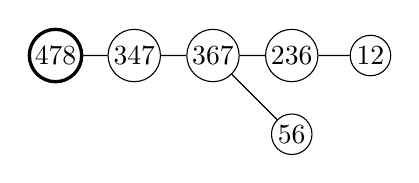
\begin{tikzpicture}
		\node[very thick, draw, circle, inner sep = 1] at (0,1) (478) {478};
		\node[draw, circle, inner sep = 1] at (1,1) (347) {347};
		\node[draw, circle, inner sep = 1] at (2,1) (367) {367};
		\node[draw, circle, inner sep = 1] at (3,1) (236) {236};
		\node[draw, circle, inner sep = 1] at (4,1) (12) {12};
		\node[draw, circle, inner sep = 1] at (3,0) (56) {56};
		\draw (478) -- (347) -- (367) -- (236) -- (12) (367) -- (56);
		\end{tikzpicture}
	\end{subfigure}
	\parbox{.3\textwidth}{\centering\begin{tabular}{c|c}Knoten&Gewicht\\\hline
			1&3\\2&1\\3&1\\4&2\\5&3\\6&2\\7&1\\8&4
		\end{tabular}}
\end{figure}
\begin{align*}
\begin{array}{|c|c|c|}
\hline
\multicolumn{3}{|c|}{12}\\\hline
\text{ }&\text{w}&\text{nodes}\\\hline
\emptyset	& 0 & \{\}\\
1			& 3 & \{1\}\\
2			& 1 & \{2\}\\\hline
\end{array}~
\begin{array}{|c|c|c|}
\hline
\multicolumn{3}{|c|}{236}\\\hline
\text{ }&\text{w}&\text{nodes}\\\hline
\emptyset	& 3 & \{1\}\\
2			& 1 & \{2\}\\
3			& 4 & \{1,3\}\\
6			& 5 & \{1,6\}\\
36			& 6 & \{1,3,6\}\\\hline
\end{array}~
\begin{array}{|c|c|c|}
\hline
\multicolumn{3}{|c|}{56}\\\hline
\text{ }&\text{w}&\text{nodes}\\\hline
\emptyset	& 0 & \{\}\\
5			& 3 & \{5\}\\
6			& 2 & \{6\}\\\hline
\end{array}~
\begin{array}{|c|c|c|}
\hline
\multicolumn{3}{|c|}{367}\\\hline
\text{ }&\text{w}&\text{nodes}\\\hline
\emptyset	& 4 & \{2,5\}\\
3			& 7 & \{1,3,5\}\\
6			& 5 & \{1,6\}\\
7			& 5 & \{2,5,7\}\\
36			& 6 & \{1,3,6\}\\\hline
\end{array}~
\begin{array}{|c|c|c|}
\hline
\multicolumn{3}{|c|}{347}\\\hline
\text{ }&\text{w}&\text{nodes}\\\hline
\emptyset	& 5 & \{1,6\}\\
3			& 7 & \{1,3,5\}\\
4			& 7 & \{1,4,6\}\\
7			& 5 & \{1,6\}\\\hline
\end{array}~
\begin{array}{|c|c|c|}
\hline
\multicolumn{3}{|c|}{478}\\ \hline
\text{ }&\text{w}&\text{nodes}\\\hline
\emptyset	& 7 & \{1,4,6\}\\
4			& 7 & \{1,4,6\}\\
7			& 5 & \{1,6\}\\
8			& 11 & \{1,3,5,8\}\\\hline
\end{array}
\end{align*}
$\rightarrow$ $MWIS = \left( 11, \{1,3,5,8\} \right)$\qed
\end{document}